\documentclass[handout]{beamer}  

%Smaller gap at between top and bottom of block when there are displayed equations
\addtobeamertemplate{block begin}{\setlength\abovedisplayskip{0pt}}
{\setlength{\belowdisplayskip}{0pt}}


\usepackage{setspace}
\linespread{1.3}
\usepackage{amssymb, amsmath, amsthm} 
\usepackage{rotating}
\usepackage{multirow}
\usepackage{graphicx}
\usepackage{synttree}
\usepackage{verbatim}
\usepackage{fancybox}
\usepackage{color}
\usepackage{tikz}
\usetikzlibrary{shapes,backgrounds}
\usepackage{hyperref}
\usetikzlibrary{trees}
\newcommand{\p}{\mathbb{P}}
\newcommand{\expect}{\mathbb{E}}


%\setbeamertemplate{blocks}[rounded][shadow=true] 
%gets rid of bottom navigation bars
\setbeamertemplate{footline}{
   \begin{beamercolorbox}[ht=4ex,leftskip=0.3cm,rightskip=0.3cm]{author in head/foot}
%    \usebeamercolor{UniBlue}
    \vspace{0.1cm}
    %\insertshorttitle \ - \insertdate 
    \hfill \insertframenumber / \inserttotalframenumber
   \end{beamercolorbox}
   \vspace*{0.1cm}
} 


%gets rid of navigation symbols
\setbeamertemplate{navigation symbols}{}


%Include or exclude the notes?
%\setbeameroption{show notes}
\setbeameroption{hide notes}


\title[Econ 103]{Economics 103 -- Statistics for Economists} 
\author[F. DiTraglia]{Francis J.\ DiTraglia}
\institute{University of Pennsylvania}
\date{Lecture 8}
\begin{document} 




%%%%%%%%%%%%%%%%%%%%%%%%%%%%%%%%%%%%%%%%

\begin{frame}[plain]
	\titlepage 
	

\end{frame} 

%%%%%%%%%%%%%%%%%%%%%%%%%%%%%%%%%%%%%%%%
\begin{frame}
\frametitle{Probability Theory}


\begin{block}{What We've Done So Far}
Axioms of probability, rules for computing probabilities of events
\end{block}

\begin{block}{What Remains}
Notion of event subsumed by that of \emph{\alert{Random Variable}}
\end{block}
\begin{block}{Random Variable}
	A more abstract way of representing a random experiment: focus only on the important information, not the irrelevant details.
\end{block}


\end{frame}
%%%%%%%%%%%%%%%%%%%%%%%%%%%%%%%%%%%%%%%%
%\begin{frame}
%\frametitle{Don't Be Surprised if You're a Little Confused}
%
%There is a conceptual hurdle involved in the transition to thinking about probabilities in terms of Random Variables. This is a point in the course where some students start to feel ``lost.'' To keep this from happening to you, it is very important to focus on the intuition and the connection to what we have already learned.
% 
%\vspace{2em}
%Don't be afraid to ask questions about this material, either in person or on Piazza. Random Variables are confusing at first, but understanding them will make the rest of the course \alert{much easier}.
%
%\end{frame}
%%%%%%%%%%%%%%%%%%%%%%%%%%%%%%%%%%%%%%%%
% \begin{frame}
% \frametitle{Why Random Variables?}
%  
% \begin{block}{Statistics}
% Use samples to learn about populations.
% \end{block}
%  
% \begin{block}{Preliminaries}
% Take population as given and then work out the probabilistic behavior of samples.
% \end{block}
%  
% \begin{block}{Random Variables as Probability Models}
% A mathematical abstraction to represent the key features of sampling.
% \end{block}
% \end{frame}
% %%%%%%%%%%%%%%%%%%%%%%%%%%%%%%%%%%%%%%%%
\begin{frame}
\frametitle{A New Way of Thinking about Populations}

\begin{itemize}
	\item \emph{No longer} think of a population as a list of $N$ objects.
	\item \emph{Represent} a population by a \alert{probability model} using the language of Random Variables.
	\item Re-express population parameters as \emph{features} of the Random Variables that \emph{represent} a population.
	\item E.g.\ if we say ``$\mu$ is the mean of a random variable $X$'' the idea is that $\mu$ is the mean of a \alert{\emph{population represented}} by the random variable $X$.
\end{itemize}


\end{frame}
%%%%%%%%%%%%%%%%%%%%%%%%%%%%%%%%%%%%%%%%
\begin{frame}
\frametitle{Why are we getting rid of population size $N$?}

 
\begin{enumerate}
	\item Don't know $N$ for real-world populations. 
	\item For sampling $N$ is irrelevant: all that matters are the \alert{\emph{relative frequencies}} in the population. 
\end{enumerate}

\begin{block}{Key Innovation}
Treat population relative frequencies as \emph{probabilities} rather than counts divided by $N$.
\end{block}
 
\begin{block}{Why Does This Make Sense?}
We defined probability as long-run relative frequency. The idea of ``long-run'' here is repeated sampling from the population.
\end{block}

\end{frame}
%%%%%%%%%%%%%%%%%%%%%%%%%%%%%%%%%%%%%%%%
\begin{frame}
\frametitle{Treating Population Relative Frequencies as Probabilities}
 
\begin{block}{Discrete Data $\Rightarrow$ Discrete Random Variables}
It's obvious what the ``right probability'' is in this case. For example if 52000 people in a population of 100000 voted for Obama, we'd represent this as a probability of $0.52$.
\end{block}

 
\begin{block}{Continuous Data $\Rightarrow$ Continuous Random Variables}
Here things are more complicated. What proportion of people have a height of exactly 62.374827 inches? To get around this problem we'll proceed by an analogy to histograms.
\end{block}

\end{frame}
%%%%%%%%%%%%%%%%%%%%%%%%%%%%%%%%%%%%%%%%

\begin{frame}

\Large The first thing to know about Random Variables is that they are neither random nor variables...

\end{frame}
%%%%%%%%%%%%%%%%%%%%%%%%%%%%%%%%%%%%%%%%
\begin{frame}
\begin{block}{Random Variable (RV)}
\emph{Fixed} function from sample space $S$ to real numbers ($X\colon S \mapsto \mathbb{R}$). Turns \emph{basic outcomes} of random experiment into \emph{numbers}.
\end{block}
 
\begin{block}{Realization}
Particular value that RV takes on, i.e.\ the result of applying the function defined by $X$ to the \emph{outcome} of the random experiment. We write $X= x$. Note that $\{X = x\}$ is an \emph{event}.
\end{block}
 
\begin{block}{Support Set}
The set of all possible realizations of a RV.
\end{block}
 
\begin{block}{Notation}
RVs denoted by capital letters, e.g.\ $X,Y,Z$, their realizations by the corresponsing lowercase letters, e.g.\ $x,y,z$.
\end{block}


\end{frame}
%%%%%%%%%%%%%%%%%%%%%%%%%%%%%%%%%%%%%%%%
%Some macros for diagrams of random variables
\def\RVraw{(-2.5,0) circle [radius=1.7]
	(-2.5,0) circle [radius=1.7]
	(2.5,0) circle [radius=1.7]
	node [above left] at (-3.75,1.25) {$S$}
	node [above right] at (3.75,1.25) {$\mathbb{R}$}
	node [above] at (0,2) {$X\colon S \mapsto \mathbb{R}$}}
%%%%%%%%%%%%%%%%%%%%%%%%%%%%%%%%%%%%%%%%
\begin{frame}
\frametitle{Random Variables}

\begin{figure}
\centering
\begin{tikzpicture}
	\draw \RVraw;
	\draw [->] (-2.5,0.5) node [below]{$o$} to [out=35,in=145] (2.5,0.5) node [below]{$x = X(o)$};
\end{tikzpicture}
\caption{A Random Variable $X$ is a fixed, i.e.\ deterministic, function that maps each basic outcome in the sample space $S$ to a real number. Here $o$ is a basic outcome and $x$ is a realization, equal to $X(o)$.}
\end{figure}


\end{frame}
%%%%%%%%%%%%%%%%%%%%%%%%%%%%%%%%%%%%%%%%
\begin{frame}
\frametitle{Important Distinction}


Although a Random Variable is a deterministic function, the \alert{\emph{values it takes on}} are random since its input, the outcome of a random experiment, is random!


\end{frame}

%%%%%%%%%%%%%%%%%%%%%%%%%%%%%%%%%%%%%%%%
\begin{frame}
\frametitle{Example: Coin Flip Random Variable}

\begin{figure}
\centering
\begin{tikzpicture}
	\draw \RVraw;
	\draw [->] (-2.5,0.75) node [below]{Tails} to [out=35,in=145] (2.5,0.75) node [below]{$0$};
	\draw [->] (-2.5,-0.75) node [above]{Heads} to [out=315,in=225] (2.5,-0.75) node [above]{$1$};
\end{tikzpicture}
\caption{This random variable maps the outcomes of flipping a coin $\{\mbox{Heads}, \mbox{Tails}\}$ to the set $\{0,1\}\subseteq \mathbb{R}$. Hence, its support is $\{0,1\}$}
\end{figure}
\end{frame}
%%%%%%%%%%%%%%%%%%%%%%%%%%%%%%%%%%%%%%%%
% \begin{frame}
% \frametitle{Why map to $\mathbb{R}$?}

% We can do math with real numbers, but we can't do math with ``Heads'' or ``Tails.'' The point is to make our lives easier at the same time as we develop a richer framework for thinking about probabilities.
% \end{frame}
% %%%%%%%%%%%%%%%%%%%%%%%%%%%%%%%%%%%%%%%%
% \begin{frame}
% 	\frametitle{Countable and Uncountable Sets}
% 	 
% 	\begin{block}{Countable}
% 	All elements can be enumerated in a list: $1, 2, 3, \hdots$. Does \emph{not} mean finite, although finite sets are countable. 
	
% 	 
% 	\emph{Examples:} any finite set, $\mathbb{N}$, $\mathbb{Z}$, $\mathbb{Q}$.
% 	\end{block}
% 	 
% 	\begin{block}{Uncountable}
% 	All elements \emph{cannot} be enumerated in a list. Implies infinite, but some infinities are larger than others!
	
% 	 
% 	\emph{Examples:} $\mathbb{R}$, any subset made up of intervals on $\mathbb{R}$
% 	 \end{block}
% \end{frame}
% %%%%%%%%%%%%%%%%%%%%%%%%%%%%%%%%%%%%%%%%
\begin{frame}
\frametitle{Types of Random Variables}
 
	\begin{block}{Discrete RVs}
	Takes on a finite or countably infinite number of different values, e.g.\  $\{-1, 0, 1\}$ or $\{0, 1, 2, 3, 4, 5, 6, \hdots ...\}$
	\end{block}
 	
	\begin{block}{Continuous RVs}
	Takes on an uncountably infinite number of different values, e.g.\ all real numbers in the interval $[0,1]$ or $(-\infty, \infty)$.
	\end{block}

	%  	
	% \vspace{1em}
	% \alert{It's possible to give a unified treatment of continuous and discrete RVs but for this class we'll treat them separately. We'll start with discrete RVs since they're simpler, but most of the ideas will carry over to continuous RVs.}
\end{frame}
%%%%%%%%%%%%%%%%%%%%%%%%%%%%%%%%%%%%%%%%

\begin{frame}

\centering \Huge Discrete Random Variables I

\end{frame}
%%%%%%%%%%%%%%%%%%%%%%%%%%%%%%%%%%%%%%%%
\begin{frame}
\frametitle{Probability Mass Function (pmf)}
 Probability that a \alert{Discrete RV} takes on the particular value $x$ as a function of $x$:
 $$p(x) = P(X =x)$$

 

\begin{alertblock}{Plug in a realization $x$, get out a probability  $p(x)$.}\end{alertblock}

 


\end{frame}
%%%%%%%%%%%%%%%%%%%%%%%%%%%%%%%%%%%%%%%%
\begin{frame}
\frametitle{Probability Mass Function for Coin Flip RV}

\begin{columns}
\column{0.25\textwidth}
$$X = \left\{ \begin{array}{l}  0, \mbox{Tails}\\ 1, \mbox{Heads}\end{array} \right.$$

\begin{eqnarray*}
	p(0) &=& 1/2\\
	p(1) &=& 1/2
\end{eqnarray*}


\column{0.75\textwidth}
\begin{figure}
\centering
\begin{tikzpicture}[scale = 1.5]
\draw [<->] (0,2) node [above]{$p(x)$} -- (0,0) -- (3,0) node [right]{$x$};
\draw [blue, thick] (0.75,0) node [black, below]{0} -- (0.75,1.5);
\draw [blue, thick] (2.25,0) node [black, below]{1} -- (2.25,1.5);
\draw [dashed, gray] (0, 1.5) node [black, left]{$1/2$} -- (3,1.5);
\draw [fill=blue] (2.25,1.51) circle [radius = 0.05];
\draw [fill=blue] (0.75,1.51) circle [radius = 0.05];
\end{tikzpicture}
\caption{Plot of pmf for Coin Flip Random Variable}
\end{figure}
\end{columns}

\vspace{3em}
\alert{Where did this come from?}

\end{frame}
%%%%%%%%%%%%%%%%%%%%%%%%%%%%%%%%%%%%%%%%


\begin{frame}
\small
\begin{figure}
\centering
\fbox{
\begin{tikzpicture}[scale=0.45]
	\draw \RVraw;
	\draw [->] (-2.5,1) node [below]{Tails} to [out=35,in=145] (2.5,1) node [below]{$0$};
	\draw [->] (-2.5,-1) node [above]{Heads} to [out=315,in=225] (2.5,-1) node [above]{$1$};
\end{tikzpicture}}
\end{figure}
 
\begin{block}{Support Set $\{0,1\}$}
The only possible realizations are $X=0$ and $X=1$
\end{block}
 
\begin{block}{Events}
Tracing the arrows backwards, $\{X=0\}$ corresponds to the event ``Tails'' while $\{X=1\}$ corresponds to the event ``Heads.''
\end{block}
 
\begin{block}{Probabilities}
Since $P(\mbox{Heads}) = P(\mbox{Tails}) = 1/2$, $P(X=0) = P(X=1) = 1/2$
\end{block}

\end{frame}
%%%%%%%%%%%%%%%%%%%%%%%%%%%%%%%%%%%%%%%%


\begin{frame}
\frametitle{Important Note about Support Sets}
Whenever you write down the pmf of a RV, it is \alert{crucial} to also write down its Support Set. Recall that this is the set of \alert{\emph{all possible realizations for a RV}}. Outside of the support set, all probabilities are zero. In other words, the pmf is \alert{only defined} on the support.

\end{frame}
%%%%%%%%%%%%%%%%%%%%%%%%%%%%%%%%%%%%%%%%
\begin{frame}
\frametitle{Properties of Probability Mass Functions}

If $p(x)$ is the pmf of a random variable $X$, then
\begin{enumerate}[(i)]
	\item $0\leq p(x) \leq 1$ for all $x$ \vspace{1em}
	\item $\displaystyle \sum_{\mbox{all } x} p(x) = 1$
\end{enumerate}

\vspace{0.75em}
where ``all $x$'' is shorthand for ``all $x$ in the support of $X$.''


 

\vspace{2em}
\begin{alertblock}{But Where Do These Come From?}
The key point is that $\{X=x\}$ is an \emph{event}. We proceed by working backwards until we are in familiar territory...
\end{alertblock}

\end{frame}
%%%%%%%%%%%%%%%%%%%%%%%%%%%%%%%%%%%%%%%%
\begin{frame}
\frametitle{Which Event Corresponds to $\{X=x_1\}$?}

\begin{figure}
	\centering
\begin{tikzpicture}[scale = 1]
	\draw \RVraw;
	\draw [blue, ultra thick] (-2.85,0) circle [radius=0.8];
	\draw node [blue, below left] at (-3,-0.8) {$A$};
	\draw [->] (-2.5,0.5) node [left]{$o_1$} to [out=25,in=150] (2.5,0.1);
	\draw [->] (-2.5,-0.5) node [left]{$o_2$} to [out=335,in=210] (2.5,-0.1);
	\draw (2.5, 0) node [right]{$x_1$};
\end{tikzpicture}
\end{figure}



Define \textcolor{blue}{$A = \{o \in S \colon X(o) = x_1\}$}. Since it is a subset of the sample space, $A$ is an event. Since $A$ contains \emph{all} the basic outcomes that map to $x_1$, \textcolor{blue}{$A = \{X=x_1\}$}, hence \textcolor{blue}{$P(A) = P(X=x_1)$}.


\end{frame}
%%%%%%%%%%%%%%%%%%%%%%%%%%%%%%%%%%%%%%%%
\begin{frame}
	\frametitle{Link Between Axioms of Probability and Random Variables}

	\begin{enumerate}
		\item We can equate $\{X=x\}$ with an event $A$ in $S$ for any realization $x$ in the support of $X$. Thus $P(X=x) = p(x)$ is a bona fide probability and
				$$0 \leq p(x) \leq 1$$
		\item Since $X$ is a \emph{function}, the events $\{X= x\}$ are \alert{mutually exclusive} and \alert{collectively exhaustive}, hence:
		$$\sum_{\mbox{all } x} p(x) = \sum_{\mbox{all } x} P(X=x) = P(S) = 1$$
	\end{enumerate}

\end{frame}

%%%%%%%%%%%%%%%%%%%%%%%%%%%%%%%%%%%%%%%%
\begin{frame}
\frametitle{Is This Possible? (A = Yes, B = No) \hfill 
\includegraphics[scale = 0.05]{./images/clicker}}

\begin{figure}
\begin{tikzpicture}
	\draw \RVraw;
		\draw [->] (-2.5,0) node [left]{$o_1$} to [out=25,in=170] (2.5,0.75) node [right]{$x_1$};
	\draw [->] (-2.5,0) to [out=335,in=190] (2.5,-0.75) node [right]{$x_2$};
\end{tikzpicture}
\caption{This diagram shows the random variable $X$ mapping the basic outcome $o_1$ to two different realizations: $x_1$ and $x_2$. Is this allowed?}
\end{figure}

\end{frame}


%%%%%%%%%%%%%%%%%%%%%%%%%%%%%%%%%%%%%%%%
\begin{frame}
\frametitle{This is NOT POSSIBLE}

\begin{figure}
\centering
\begin{tikzpicture}[scale = 0.8]
	\draw \RVraw;
		\draw [->] (-2.5,0) node [left]{$o_1$} to [out=25,in=170] (2.5,0.75) node [right]{$x_1$};
	\draw [->] (-2.5,0) to [out=335,in=190] (2.5,-0.75) node [right]{$x_2$};
\end{tikzpicture}
\end{figure}

\begin{itemize}
	\item A function cannot map a single input to two different outputs! You may know this as the ``vertical line test.''
	\item We have to rule this situation out since it would mean that $\{X = x_1\}$ and $\{X = x_2\}$ are \emph{not mututally exclusive}.
\end{itemize}

\end{frame}


%%%%%%%%%%%%%%%%%%%%%%%%%%%%%%%%%%%%%%%%
\begin{frame}
\frametitle{Is This Possible? (A = Yes, B = No) \hfill 
\includegraphics[scale = 0.05]{./images/clicker}}

\begin{figure}
\centering
\begin{tikzpicture}[scale = 0.8]
	\draw \RVraw;
		\draw [->] (-2.5,0) node [left]{$o_1$} to [out=25,in=170] (2.5,0.75) node [right]{$x_1$};
	\draw (-2.5,-0.75) node [right]{$o_2$};
\end{tikzpicture}
\caption{This diagram shows the random variable $X$ mapping the basic outcome $o_1$ to the realization $x_1$. The basic outcome $o_2$ doesn't get mapped anywhere. Is this allowed?}
\end{figure}

\end{frame}
%%%%%%%%%%%%%%%%%%%%%%%%%%%%%%%%%%%%%%%%
\begin{frame}
\frametitle{This is NOT POSSIBLE}



\begin{figure}
\begin{tikzpicture}
	\draw \RVraw;
		\draw [->] (-2.5,0) node [left]{$o_1$} to [out=25,in=170] (2.5,0.75) node [right]{$x_1$};
	\draw (-2.5,-0.75) node [right]{$o_2$};
\end{tikzpicture}
\end{figure}
\begin{itemize}
	\item A function associates \emph{every} value in its domain with a value in its range: $o_2$ has to map to something!
	\item We have to rule this situation out since it would mean that the events $\{X = x\}$ are \emph{not collectively exhaustive}. 
\end{itemize}


\end{frame}

%%%%%%%%%%%%%%%%%%%%%%%%%%%%%%%%%%%%%%%%

\begin{frame}
\frametitle{Cumulative Distribution Function (CDF)}
\framesubtitle{This Def.\ is \alert{the same} for continuous RVs.}

The CDF gives the probability that a RV $X$ \alert{does not exceed} a specified threshold $x_0$, as a function of $x_0$
	$$F(x_0) = P(X \leq x_0)$$


 

\begin{alertblock}{Important!}
The threshold $x_0$ is allowed to be \emph{any real number}. In particular, it doesn't have to be in the support of $X$! 
\end{alertblock}

\end{frame}
%%%%%%%%%%%%%%%%%%%%%%%%%%%%%%%%%%%%%%%%


\begin{frame}
\frametitle{CDF of Coin Flip Random Variable}
\begin{columns}
\column{0.4\textwidth}
$$X = \left\{ \begin{array}{l}  0, \mbox{Tails}\\ 1, \mbox{Heads}\end{array} \right.$$

\begin{eqnarray*}
	F(x_0) = \left\{\begin{array}{ll} 0,& x_0 < 0\\ \frac{1}{2}, &0\leq x_0 < 1\\ 1,& x_0 \geq 1\end{array}\right.
\end{eqnarray*}


\column{0.6\textwidth}
\begin{figure}
\centering
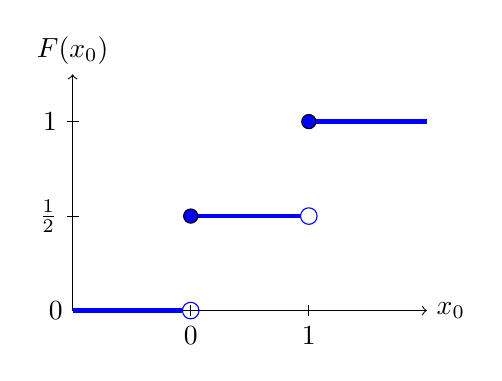
\begin{tikzpicture}[scale = 1.5]
\draw [<->] (0,2) node [above]{$F(x_0)$} -- (0,0) -- (3,0) node [right]{$x_0$};
\draw (-0.05, 1.6) node [black, left]{$1$} -- (0.05,1.6);
\draw (-0.05, 0.8) node [black, left]{$\frac{1}{2}$} -- (0.05,0.8);
\draw [blue, ultra thick] (0,0) -- (0.93,0);
\draw [blue, ultra thick] (1,0.8) -- (1.93,0.8);
\draw [blue, ultra thick] (2,1.6) -- (3,1.6);
\draw (1,-0.05) node [black, below]{0} -- (1,0.05);
\draw (2,-0.05) node [black, below]{1} -- (2,0.05);
\draw (0,0) node [black, left]{$0$};
\draw [blue] (1,0) circle [radius = 0.07];
\draw [fill = blue] (1,0.8) circle [radius = 0.06];
\draw [blue] (2,0.8) circle [radius = 0.07];
\draw [fill = blue] (2,1.6) circle [radius = 0.06];
\end{tikzpicture}
\caption{ CDF for Coin Flip Random Variable}
\end{figure}
\end{columns}

\vspace{3em}
\hfill\alert{\large Where did we get this from?}
\end{frame}
%%%%%%%%%%%%%%%%%%%%%%%%%%%%%%%%%%%%%%%%
\begin{frame}
\frametitle{Discrete RVs: Sum the pmf to get the CDF}
\begin{center}
	\alert{$$\boxed{F(x_0) = \sum_{x\leq x_0} p(x)}$$}
\end{center}

\small
 
\begin{block}{Proof}
Use the fact that the events $\{X = x\}$ are mutually exclusive:
	$$F(x_0) = P(X \leq x_0)=   P\left(\bigcup_{x\leq x_0}\{X = x\}\right) =   \sum_{x \leq x_0} P(X = x) =   \sum_{x \leq x_0} p(x)$$
\end{block}

\end{frame}
%%%%%%%%%%%%%%%%%%%%%%%%%%%%%%%%%%%%%%%%


\begin{frame}[t]
	% \frametitle{Sum the pmf to get the CDF}
	% \framesubtitle{Coin-Flip Random Variable}

\begin{columns}[t]
	\column{0.48\textwidth}
	\begin{block}{Probability Mass Function}
	\begin{figure}
\centering
\begin{tikzpicture}[scale = 1.2]
\draw [<->] (0,2) node [above]{$p(x)$} -- (0,0) -- (3,0) node [right]{$x$};
\draw [blue, thick] (0.75,0) node [black, below]{0} -- (0.75,1.5);
\draw [blue, thick] (2.25,0) node [black, below]{1} -- (2.25,1.5);
\draw [dashed, gray] (0, 1.5) node [black, left]{$1/2$} -- (3,1.5);
\draw [fill=blue] (2.25,1.51) circle [radius = 0.05];
\draw [fill=blue] (0.75,1.51) circle [radius = 0.05];
\end{tikzpicture}
\end{figure}
\begin{eqnarray*}
	p(0) &=& 1/2\\
	p(1) &=& 1/2
\end{eqnarray*}
	\end{block}

	\column{0.48\textwidth}
	\begin{block}{Cumulative Dist.\ Function}
\begin{figure}
\centering
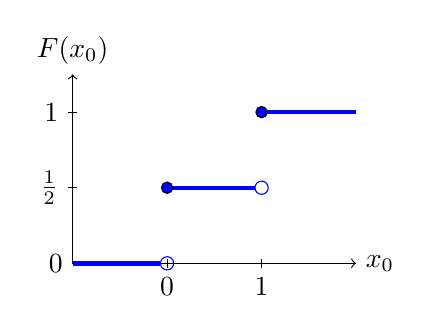
\begin{tikzpicture}[scale = 1.2]
\draw [<->] (0,2) node [above]{$F(x_0)$} -- (0,0) -- (3,0) node [right]{$x_0$};
\draw (-0.05, 1.6) node [black, left]{$1$} -- (0.05,1.6);
\draw (-0.05, 0.8) node [black, left]{$\frac{1}{2}$} -- (0.05,0.8);
\draw [blue, ultra thick] (0,0) -- (0.93,0);
\draw [blue, ultra thick] (1,0.8) -- (1.93,0.8);
\draw [blue, ultra thick] (2,1.6) -- (3,1.6);
\draw (1,-0.05) node [black, below]{0} -- (1,0.05);
\draw (2,-0.05) node [black, below]{1} -- (2,0.05);
\draw (0,0) node [black, left]{$0$};
\draw [blue] (1,0) circle [radius = 0.07];
\draw [fill = blue] (1,0.8) circle [radius = 0.06];
\draw [blue] (2,0.8) circle [radius = 0.07];
\draw [fill = blue] (2,1.6) circle [radius = 0.06];
\end{tikzpicture}
\end{figure}
\begin{eqnarray*}
	F(x_0) = \left\{\begin{array}{ll} 0,& x_0 < 0\\ \frac{1}{2}, &0\leq x_0 < 1\\ 1,& x_0 \geq 1\end{array}\right.
\end{eqnarray*}
	\end{block}
\end{columns}
\end{frame}

%%%%%%%%%%%%%%%%%%%%%%%%%%%%%%%%%%%%%%%%

\begin{frame}
\frametitle{Properties of CDFs}
\framesubtitle{These are also true for continuous RVs.}
	\begin{enumerate}
		\item $\lim_{x_0 \rightarrow \infty} F(x_0) = 1$
		\item $\lim_{x_0 \rightarrow -\infty} F(x_0) = 0$
		\item Non-decreasing: $x_0 < x_1 \Rightarrow F(x_0)\leq F(x_1)$
		\item Right-continuous (``open'' versus ``closed'' on prev.\ slide)
	\end{enumerate}
	
	
	 
	
	
\vspace{1em}
\begin{alertblock}{Since $F(x_0) = P(X\leq x_0)$,  we have $0\leq F(x_0)\leq 1$ for all $x_0$}\end{alertblock}
\end{frame}
%%%%%%%%%%%%%%%%%%%%%%%%%%%%%%%%%%%%%%%%

\begin{frame}
\frametitle{Bernoulli Random Variable -- Generalization of Coin Flip}
\small
\begin{block}{Support Set}
$\{0,1\}$ -- 1 traditionally called ``success,'' 0 ``failure''
\end{block}

\begin{block}{Probability Mass Function}
	\begin{eqnarray*}
		p(0) &=& 1-p\\
		p(1) &=& p
	\end{eqnarray*}

	\begin{block}{Cumulative Distribution Function}
\begin{eqnarray*}
	F(x_0) = \left\{\begin{array}{ll} 0,& x_0 < 0\\ 1-p, &0\leq x_0 < 1\\ 1,& x_0 \geq 1\end{array}\right.
\end{eqnarray*}
\end{block}
\end{block}

\end{frame}
%%%%%%%%%%%%%%%%%%%%%%%%%%%%%%%%%%%%%%%%
\begin{frame}
	\frametitle{\href{http://glimmer.rstudio.com/fditraglia/binom_cdf/}{http://glimmer.rstudio.com/fditraglia/binom\_cdf/}}
\framesubtitle{Set the second slider to 1 and play around with the others.}

\begin{figure}
	\fbox{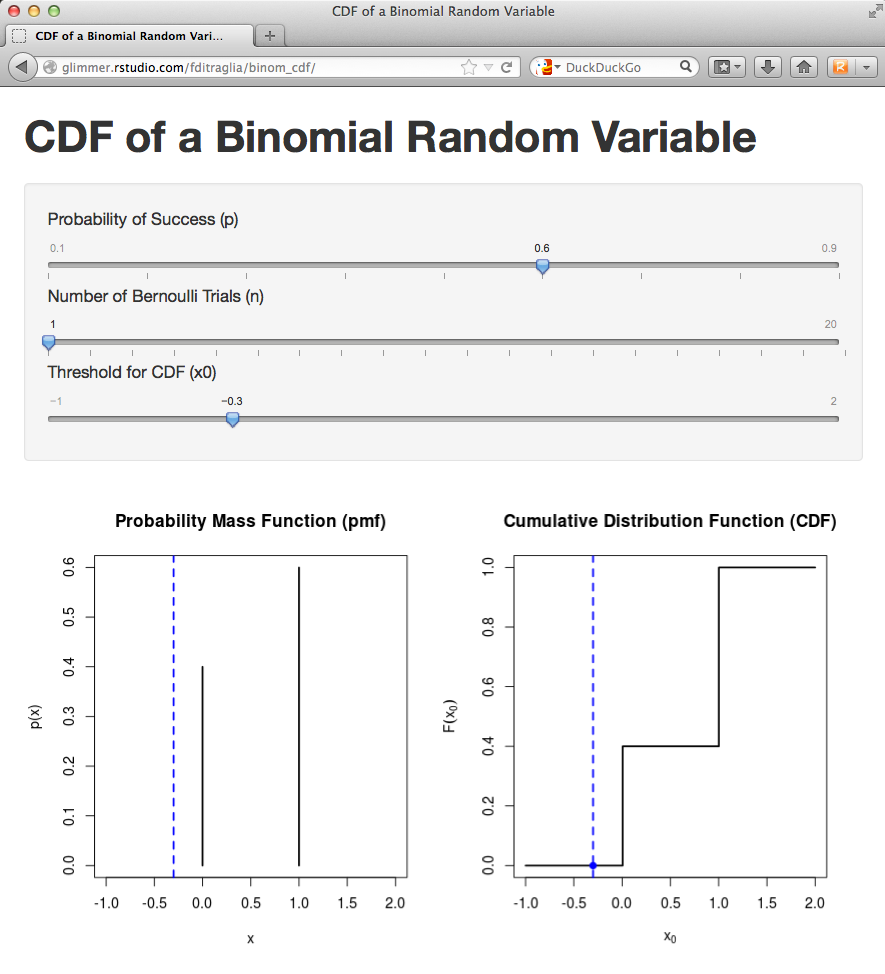
\includegraphics[scale = 0.2]{./images/binom_cdf_screenshot}}
\end{figure}

\end{frame}


%%%%%%%%%%%%%%%%%%%%%%%%%%%%%%%%%%%%%%%%
% \begin{frame}
% Notice that when I defined the Bernoulli Random Variable on the previous slide \emph{\alert{I didn't say anything about the random experiment in the background.}} There's no problem with this, in fact it is how we'll proceed from now on: talking about random variables without being explicit about the random experiment that gives rise to them.

% \vspace{1em}

%  

%  \begin{block}{Why?} 
%  There is an unlimited number of random experiments that give rise to the same random variable. We can study \emph{\alert{all of them at the same time}} by simply studying the random variable that represents them.
%   \end{block} 
% \end{frame}
% %%%%%%%%%%%%%%%%%%%%%%%%%%%%%%%%%%%%%%%%
\begin{frame}
\frametitle{Average Winnings Per Trial \hfill 
\includegraphics[scale = 0.05]{./images/clicker}}
If the realizations of the coin-flip RV were \alert{payoffs}, how much would you expect to win per play \emph{on average} in a long sequence of plays?
$$X = \left\{ \begin{array}{l}  \$0, \mbox{Tails}\\ \$1, \mbox{Heads}\end{array} \right.$$
\end{frame}
%%%%%%%%%%%%%%%%%%%%%%%%%%%%%%%%%%%%%%%%

\begin{frame}
\frametitle{Fair Price \hfill 
\includegraphics[scale = 0.05]{./images/clicker}}
If I were \emph{bankrolling} a long sequence of trials of this game, how much should I charge per play so that I break even in the long run?
$$X = \left\{ \begin{array}{l}  \$0, \mbox{Tails}\\ \$1, \mbox{Heads}\end{array} \right.$$
\end{frame}
%%%%%%%%%%%%%%%%%%%%%%%%%%%%%%%%%%%%%%%%


\begin{frame}
\centering \Huge Expected Value: Probability-Weighted Average of Realizations

\end{frame}
%%%%%%%%%%%%%%%%%%%%%%%%%%%%%%%%%%%%%%%%
\begin{frame}
\frametitle{Expected Value (aka Expectation)}
The expected value of a discrete RV $X$ is given by
	$$E[X] = \sum_{\mbox{all} \; x} x \cdot p(x)$$
	
 
	
	\vspace{2em}
\begin{alertblock}{Treating the random variable $X$ as a probability model for a population, we equate $E[X]$ with the population mean $\mu$.}\end{alertblock}
\end{frame}
%%%%%%%%%%%%%%%%%%%%%%%%%%%%%%%%%%%%%%%%
\begin{frame}
\frametitle{Expected Value of Bernoulli Random Variable\hfill 
\includegraphics[scale = 0.05]{./images/clicker}}

Suppose $p = 1/4$ since you can only enter numeric results on the clicker.
$$X = \left\{ \begin{array}{l}  0, \mbox{Failure: } 1-p\\ 1, \mbox{Success: } p\end{array} \right.$$

\pause
\vspace{2em}
 
$$\sum_{\mbox{all} \; x} x \cdot p(x) = 0 \cdot (1-p) + 1 \cdot p = p$$
\end{frame}
%%%%%%%%%%%%%%%%%%%%%%%%%%%%%%%%%%%%%%%%


\end{document}
